\chapter{\label{chapter:implementation}Hellfire Hypervisor - An Implementation Using MIPS Hardware-assistance}

This chapter presents a hypervisor implementation based on the virtualization model discussed in Section \ref{chapter:vtmodel}. This implementation was partially built by Zampiva \cite{samir2013} during his master degree, and finished during the development of this dissertation. Focused on full-virtualization, as proposed by the model, this implementation supports the MIPS virtualization extensions (MIPS VZ). The target processor is the M5150 that supports two-level TLBs, thus, it allows memory isolation at both the hypervisor and guest OS levels. Additionally, this chapter shows how software design decisions based on hardware-assisted virtualization associated with embedded systems characteristics result in a simpler hypervisor. Section \ref{chapter5:m5150} gives a brief description of the MIPS M5150 processor core. Section \ref{section:architecture} describes the software architecture of the hypervisor implementation. Section \ref{section5:vmm} explains the memory virtualization strategy adopted. Finally, Section \ref{section5:interrupt} describes the fast interrupt delivery mechanism supported by the hypervisor. 

\section{The M5150 processor}
\label{chapter5:m5150}

The M5150 processor was released by the end of 2013 and was one of the first cores based on the MIPS32 Release 5 (MIPS32r5) specification. It is a fully synthesizable MIPS processor designed for embedded applications. The main features of the processor are: single-core, 5-stage pipeline, 32-bit address and data paths, MIPS32 and microMIPS ISA \cite{micromipsISA}, 16 or 32 dual-entry joint Translation Lookaside Buffer (TLB) with variable page sizes, Multiply/Divide Unit, Floating Point Unit (FPU), upto 16 general purpose register shadow sets (copies of the normal GPR to avoid the need to save and restore them on entry to high-priority interrupts or exceptions) and Virtualization Module Support (MIPS VZ). Additionally, as part of the virtualization module, the core has two COP0 instances: one for the guest OS and the other exclusive to the hypervisor. Moreover, in the M5150 terminology the COP0 state for the guest OS is called guest-context while the COP0 state for the hypervisor is called root-context of the processor.

\subsection{MIPS32's Memory Model}

Figure \ref{fig:mips_memory} depicts the memory model of the MIPS32 processor family. The memory map for processors that implement TLB is different from processors with fixed mapping. For example, the M5100 processor does not implement the TLB on the guest's level. Thus, only the hypervisor has control over the virtual memory. The M5100 is designed for guests without TLB support. The MIPS-VZ module always requires the root-context TLB. For the purpose of this dissertation, only the memory model of the M5150 processor with two-stage TLB is presented. 

The MIPS32 core has 4 gigabytes (GB) of virtual memory space and supports 4GB of physical memory. The virtual memory space is divided into four segments for different purposes. The kuseg support 2GB of virtual address range and starts at 0x0000\_0000. It is designed for user applications and can be mapped through the TLB anywhere in the physical memory. The kuseg can be accessed from kernel or user-modes. The segments kseg0 and kseg1 are designed for OS's code and data. It only can be accessed from kernel-mode. Access to these segments from user-mode will cause an address error exception. Both segments are directly mapped to the lower 512 megabytes (0.5GB) of the physical memory. For example, the addresses 0x8000\_0000 and 0xA000\_0000 are mapped to the physical address 0x0000\_0000. However, the kseg1 does not support cache and is used during boot time and for memory-mapped I/O. The last two segments, kseg2 and kseg3, are accessible only in kernel-mode and can be mapped anywhere in the physical memory. These segments were intended to execute programs in supervisor mode. However, it took many years from the conception of MIPS32 before the virtualization in these processors could take place. Additionally, the Linux Kernel uses these segments as high kernel memory. 

\begin{figure}[!hbtp]
	\centering
	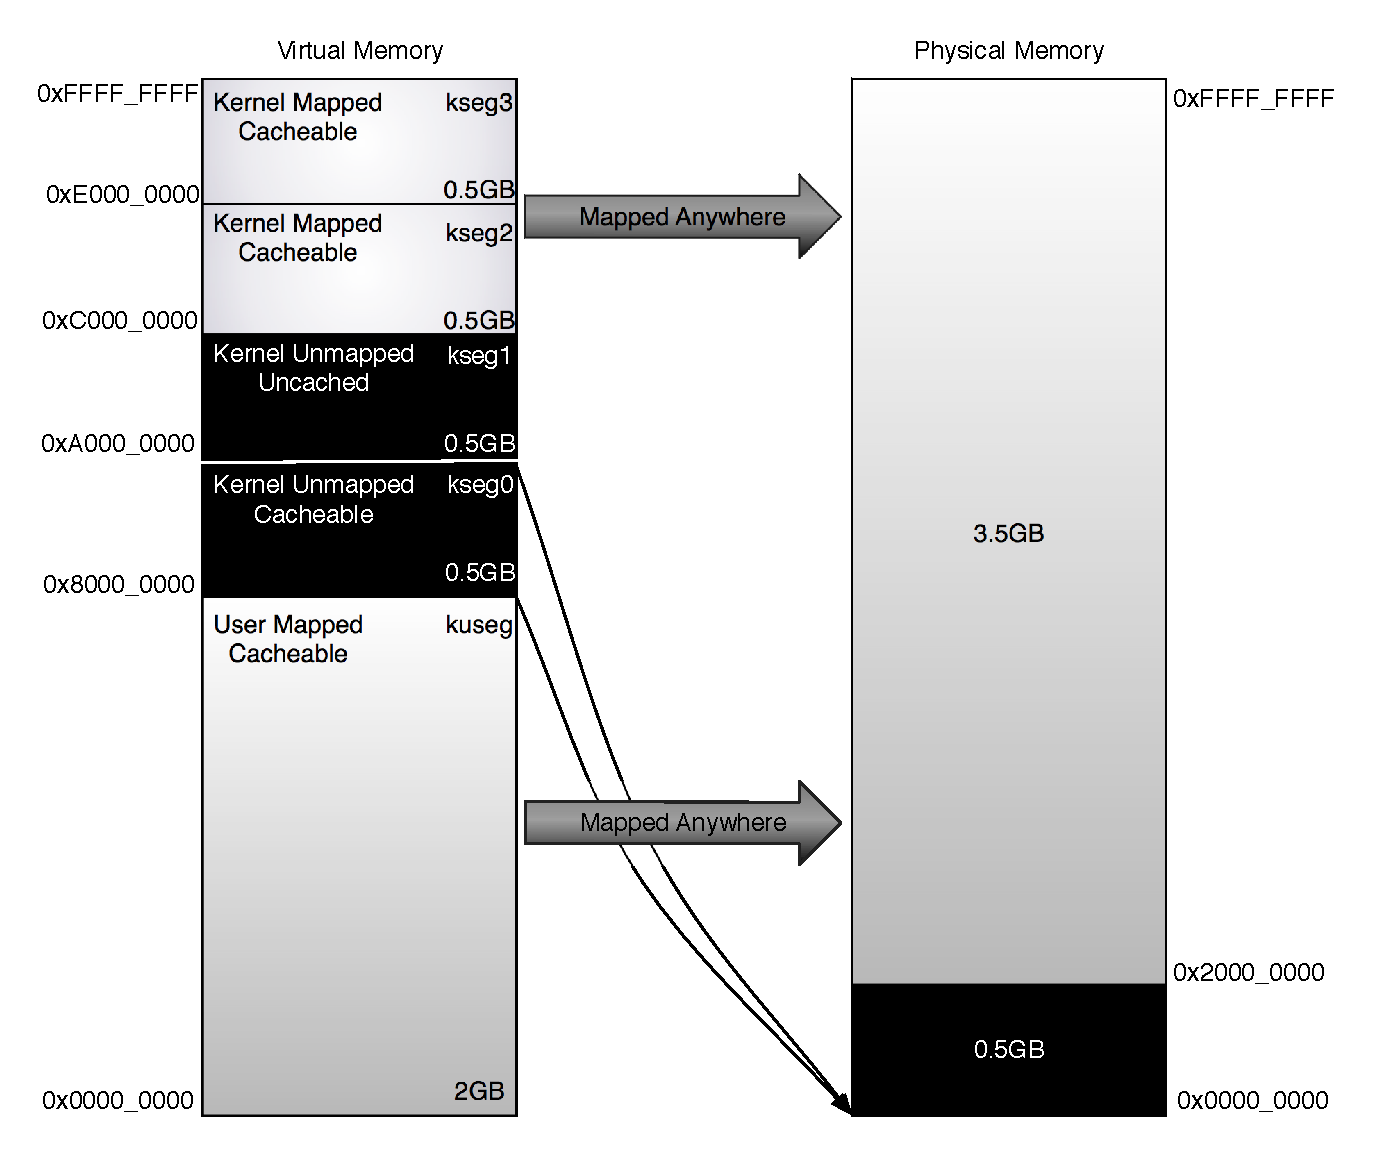
\includegraphics[width=0.5\textwidth]{chapter5/figures/mips_memory_map}
	\caption{MIPS32 memory map.}
	\label{fig:mips_memory}
\end{figure}

%\section{Hypervisor Memory Organization}


\section{Software Architecture}
\label{section:architecture}

The source code of our hypervisor was written mainly in the C programming language, but some hardware abstraction layer (HAL) parts were written in assembly. For implementation, debug and simulation purposes it was used the MIPS Instruction Accurate Simulator (IASim), which is a hardware simulator for MIPS processors able to simulate an entire platform, and based on the OVSim. However, during the development of this dissertation, only the M5150 processor, serial port and RAM memory models were available. IASim performs fast simulation aiming to deliver a virtual platform for embedded software development without the need of the real hardware platform. For better accuracy, all performance tests were performed on the SEAD-3 \cite{sead32010} development platform board, as detailed in the Chapter \ref{chapter6:evaluation}.

Figure \ref{fig:blockdiagram} shows the block diagram of hypervisor software implementation. It is composed of a hardware abstraction layer (HAL),
real-time and best-effort schedulers, dispatcher, VCPU manager, VM instantiation and toolkit. 

\begin{figure}[!hbtp]
	\centering
	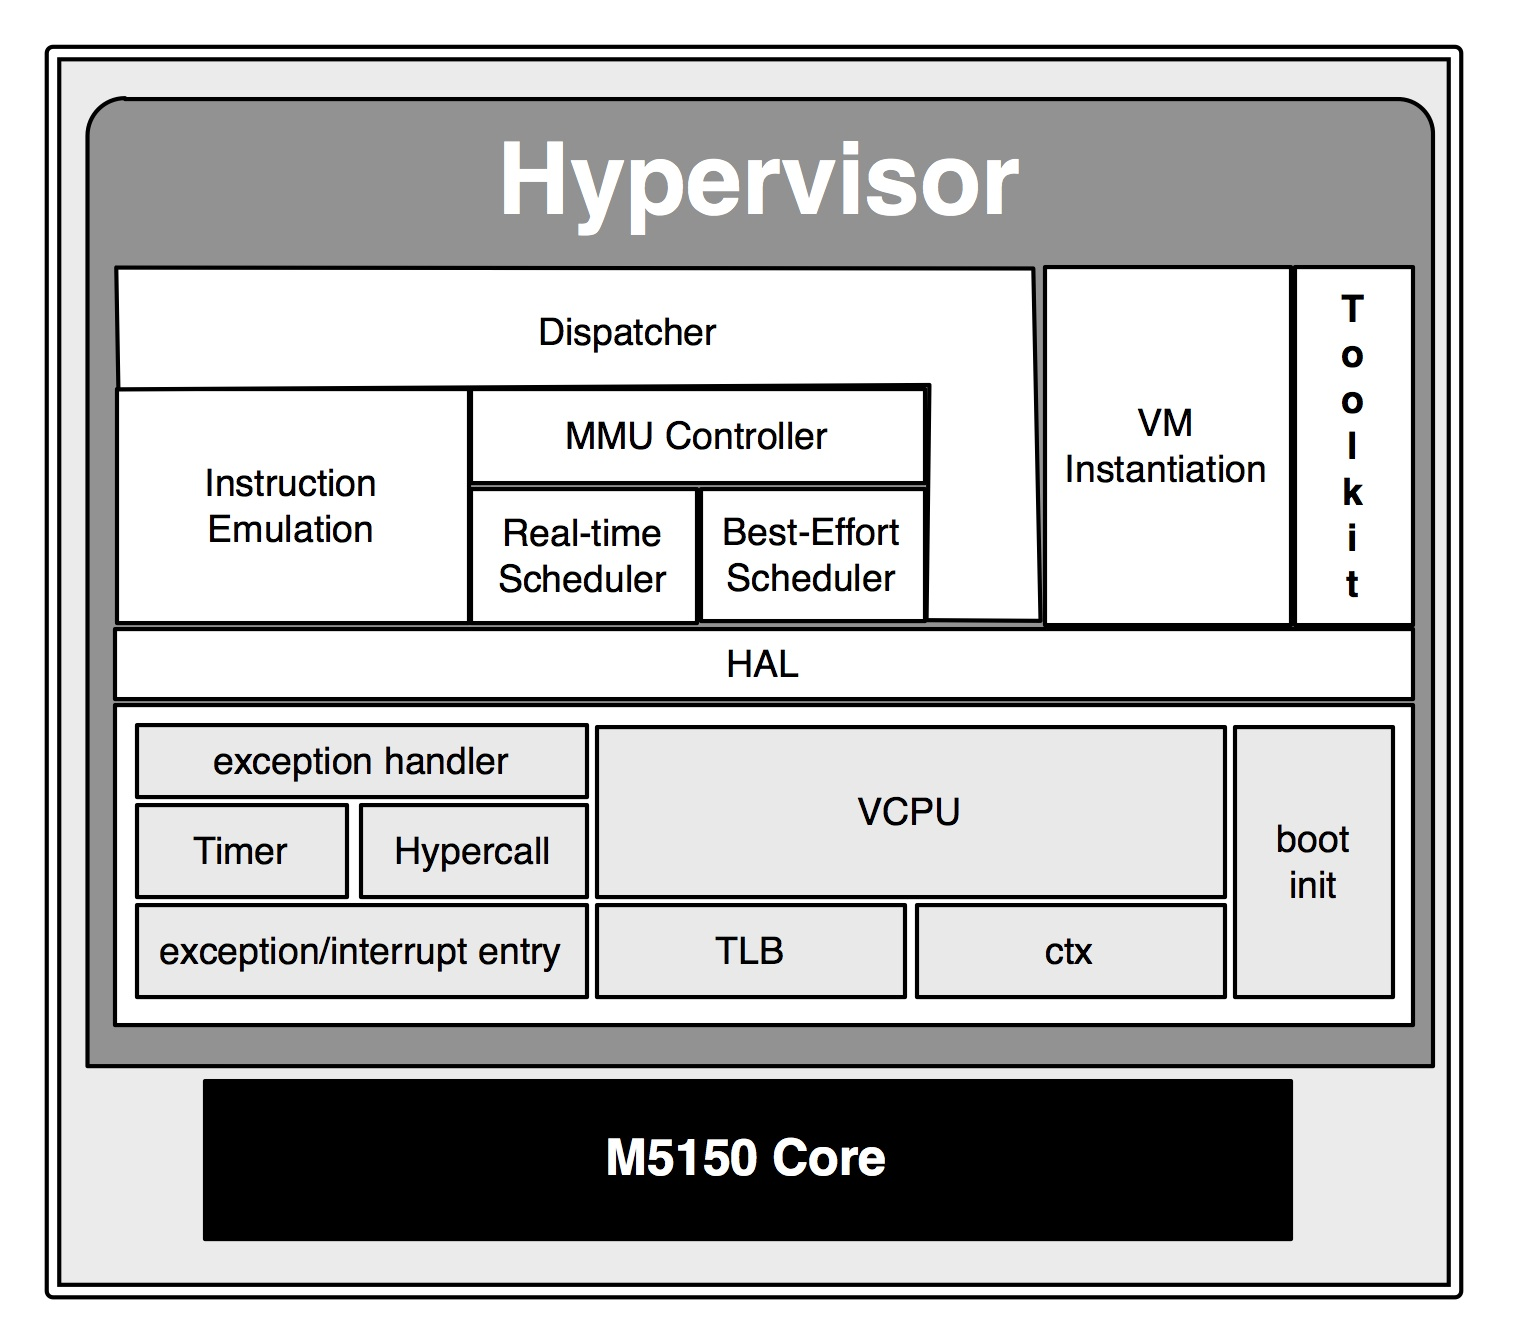
\includegraphics[width=0.5\textwidth]{chapter5/figures/hyperLayerView}
	\caption{Hypervisor's software block diagram.}
	\label{fig:blockdiagram}
\end{figure}

The HAL implements the low-level application programming interface (API) used to isolate higher layers from further hardware details. Some HAL parts were written in MIPS assembly language due to the necessity of use specific COP0 access, TLB or cache control instructions. After reset, the M5150 processor starts the instruction fetch at address 0xBFC0\_0000 in the kseg1 memory segment (non-cacheable). For a stand-alone boot process, e.g., when a boot-loader software is not present, the boot init code is placed at this address to be the first code executed after reset. This code must configure the processor accordingly and copy the hypervisor code to a cacheable memory area, in this case, the kseg0 memory segment. This boot process is used with the IASim. In the SEAD-3, the native bootloader (Yammon) is used to configure the processor and copy the hypervisor directly to the kseg0 segment. Thus, avoiding the use of the hypervisor's boot-init code. 

The real-time and best-effort schedulers are responsible for implementing the Earliest Deadline First (EDF) and best-effort round-robin scheduler algorithms for scheduling the RT-VCPUs and BE-VCPUs, respectively. The scheduler module can be easily substituted by any other algorithm. During timer interrupt handling, the hypervisor invokes the scheduler module that manages the VCPU's queues returning to the scheduled VCPU. Consequently, the dispatcher is responsible for dispatching the chosen VCPU to the physical CPU. Thus, the dispatcher uses the HAL interface to write onto the correct CPU's registers. 

The instruction emulation module is needed to emulate instructions that cannot be directly executed by the guest OS, e.g., write to specific bits of the COP0 that change the overall processor behavior as the reduced power mode bit in the status register. As a result of the MIPS-VZ module, a minimal number of instructions need to be emulated. %Subsection \ref{subsection6:impactpriv} describes the remaining instructions emulated during the boot process of the Linux and Hellfire OSs. 

The VM instantiation module is used during the hypervisor's initialization process to configure and start up the VMs. Finally, the toolkit module is a collection of software tools such as linked-list and UNIX compatible libraries. 

\subsection{Virtual Machine and Virtual CPU Software Abstraction}
\label{chapter5:vcpu_abstration}

A virtual machine must create the abstraction of a different hardware set from the original hardware platform. This different view consists of a subset of the real platform, like a compatible subset of the processor or a small amount of the entire memory. Additionally, the virtual machine can emulate hardware subsets that do not exist in the underlying hardware. KVM uses Qemu for this purposes. Pragmatically, a VM is a data structure that keeps all information necessary to control the guest execution. The VM data structure is showed in details in Appendix \ref{appendix:vm}. Typically, this data structure is kept for each guest OS. In this implementation, the VMs are allocated dynamically during the hypervisor initialization. Thus, the hypervisor's kernel uses the control information kept in these data structures to control the guest behaviors. 

Virtual CPU is an abstraction of the real CPU used to keep the last state of the CPU's registers during a context-switching. Similar to VMs, VCPUs are represented by a data structure in memory and are dynamically created during the hypervisor’s initialization. The VCPU data structure is showed in details in Appendix \ref{appendix:vcpu}. VCPUs are the execution unity of the VMs, each one represents a different execution thread. Thus, the level of concurrence in a VM depends on the number of VCPUs associated with it and the level of concurrence in the hypervisor is directly related to the total number of VCPUs in the system. There is no performance improvements if multiple VCPUs are given to a VM on a single-core processor, instead, the context-switching overhead will cause performance penalties. Thus, this implementation does not support multiple VCPUs for a VM, since the target processor is single-core. 


\section{CPU Virtualization Strategy}

The virtualization model described in the Chapter \ref{chapter:vtmodel} suggests full-virtualization of the CPU. VHH \cite{aguiar2013} implements full-virtualization of the CPU using a trap-and-emulate strategy (see Section \ref{section:vhh}) causing frequent hypervisor interventions, since all privileged instructions result in traps. This hypervisor implementation takes advantage of the hardware-assisted virtualization of the M5150 processor core. As a result, a hypervisor able to execute guest OSs with minimal intervention is expected. This section describes how the hypervisor uses the MIPS-VZ module to avoid traps. 

The MIPS-VZ module allows the hypervisor to use a different hardware configuration for each guest. Thus, the virtualized system can support software from different hardware platforms by running guests with different configurations. Additionally, the guest OSs can have features and capabilities that are different from the host processor and other guests. These different views are possible because the hypervisor can determine what processor feature subset is accessible from the guest-context. In root-context, the hypervisor configures the GuestCtl0 (guest control register 0) register that controls what privileged features can be accessed from the guest mode. 
Using the GuestCtl0 register, the designers can choose fewer hypervisor interventions, consequently less control over the processor hardware. Alternatively, they can opt for more hypervisor interventions that give them better hardware control. Some virtualized systems require more accurate hardware control, e.g., when guest OSs wish to configure different cache algorithms. In this case, the hypervisor will keep the cache instructions privileged and control the cache operation. This hypervisor implementation is focused on avoiding hypervisor interventions during guest executions as much as possible. Thus, reducing overhead and improving real-time behavior.  Table \ref{table5:guestctl0} summarizes the configurable processor features.  First, the hypervisor gives general access to the coprocessor 0 (CP0) using the bit 28 of the GuestCtl0 register. However, some features in the CP0 remain privileged. Thus, the hypervisor allows access to the cache instructions, setting the CG field (bit 24), which allows the guest to configure the cache algorithms. Still, guest OSs are allowed to have access to the config 0 through config 7 registers. The config register set specifies various configuration and capability information. Most of the fields in the config registers are initialized by hardware during the exception reset process, or they have constant values \cite{m5150}. When the hypervisor wishes to give a different view of the system configuration to a certain guest OS, it must keep the config registers privileged. Thus, reads to this registers in a guest-context will trap the hypervisor that performs a trap-and-emulate strategy. The config registers are unprivileged in guest-context when the bit 23 of the GuestCtl0 register is set. Finally, the guest OSs can directly access  the timer registers. Timer virtualization is explained in Subsection \ref{subsection5:timervz}.

\begin{table}[!hbtp]
\centering
\caption{GuestClt0 register fields. These bits are used to control the hardware accessibility by the guest OS.}
\label{table5:guestctl0}
\begin{tabular}{lll}
\hline
\hline
\multicolumn{2}{c}{\textbf{Fields}}                                   & \multicolumn{1}{c}{\multirow{2}{*}{\textbf{Description}}} \\ %\cline{1-2}
\multicolumn{1}{c}{\textbf{Name}} & \multicolumn{1}{c}{\textbf{bits}} & \multicolumn{1}{c}{}                                      \\ \hline 
CP0                               & 28                                & Guest access to coprocessor 0.                            \\
AT                                & 26-27                             & Guest Address Translation control.                        \\
GT                                & 25                                & Guest Timer register access.                              \\
CG                                & 24                                & Cache Instruction Guest-mode enable.                      \\
CF                                & 23                                & Config register access.                                   \\ \hline
\end{tabular}
\end{table}


Despite the MIPS-VZ module support, some registers or specific bits of the registers always remain privileged. For example, the reduced power mode bit in the status register will always trap the hypervisor on guest write attempts. A VM should not have direct control of the processor performance or any other feature that could disrupt the execution of other VMs. Another reason to keep certain registers privileged is to give a different view of the system to a certain guest OS, as performed by the config registers. The same case applies to the processor identification (PID) register. When the guest OS is trying to identify the processor, the hypervisor can return a different processor identification. For example, in the M5150 processor the hypervisor can return the 4Kc processor identification limiting the guest to a compatible processor subset. %Subsection \ref{subsection6:impactpriv} presents the impact performance results for the remaining privileged instructions.

The hypervisor can keep different views of the hardware to different VMs modifying the desired fields of the GuestCtl0 register during context-switching. Thus, the only hypervisor requirement is to keep an individual copy of the GuestCtl0 register in the VM's software control structure for each guest OS. This hypervisor implementation keeps direct access to all features described in Table \ref{table5:guestctl0}. 


\subsection{Best-effort and real-time scheduler algorithms}
\label{subsection:best-effort-edf}

The hypervisor implements both Earliest Deadline First (EDF) ~\cite{edf} and best-effort (round-robin) policies to deal with RT-VCPUs and BE-VCPUs, respectively. The EDF has higher execution priority than the best-effort scheduler. The latter  will not suffer from starvation since the implementation counts on time reservation for it. The EDF scheduler requires the deadline (D), period (P), and capacity (C) real-time parameters, which are received from the hypercall HCALL\_RT\_CREATE\_APP, as explained in Section \ref{subsection4:services}. For the sake of simplicity, BE-VCPUs and RT-VCPUs are kept in different software queues.

\begin{figure}[!hbtp]
	\centering
	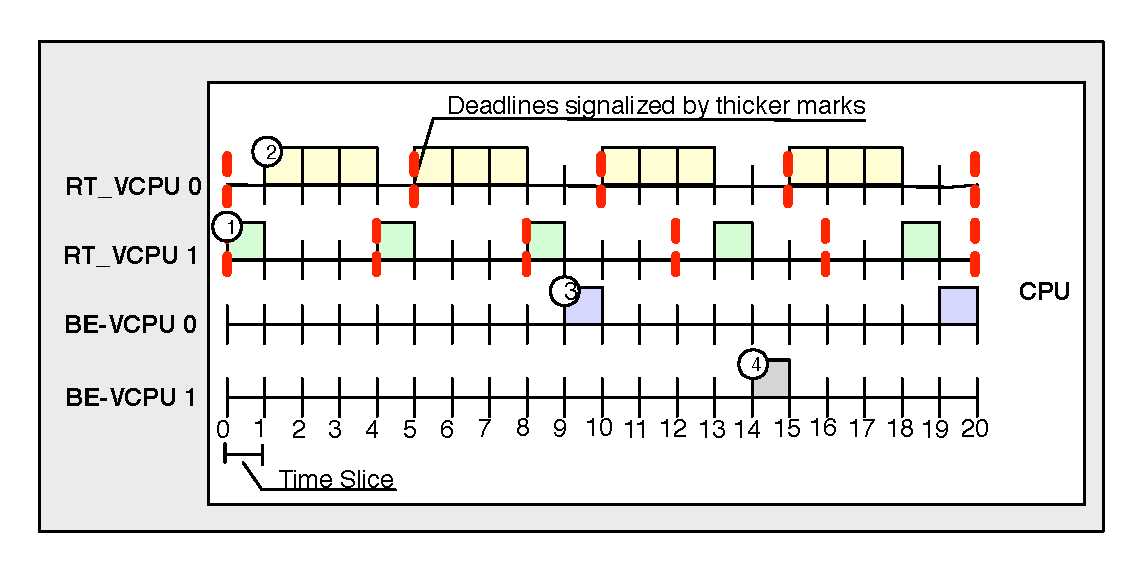
\includegraphics[width=0.7\textwidth]{chapter5/figures/tasks_scheduler_line}
	\caption{Example of the scheduling strategy to combine the EDF and best-effort schedulers.}
	\label{fig5:task_scheduler_line}
	\vspace{-0.5cm}
\end{figure}


Figure \ref{fig5:task_scheduler_line} illustrates the scheduling strategy where both EDF and best-effort schedulers cooperate to increase the CPU utilization. Assuming the execution of two BE-VCPUs and two RT-VCPUs with the following real-time parameters:

\begin{itemize}
    \item RT-VCPU 0: period = 5, capacity = 3 and deadline = 5;
    \item RT-VCPU 1: period = 4, capacity = 1 and deadline = 4.
\end{itemize}

The BE-VCPUs have the same priority. The scheduling scenario during 20 time slices can be viewed in Figure \ref{fig5:task_scheduler_line}. Each RT-VCPU is scheduled according to the EDF policy. Thus, RT-VCPU 1 executes in the first quantum as shown in (1). Next the RT-VCPU 2 executes three quanta, according to (2). In quantum 9, BE-VCPU 0 is executed for the first time because there was not any RT-VCPU ready to execute in this time slice (see (3)). Finally, The BE-VCPU 1 is executed for the first time on quantum 14 according to (4). Thus, when executed concurrently, BE-VCPUs will only execute when the RT-VCPUs are not ready to execute. An amount of CPU time can be reserved for best-effort VMs to avoid starvation. The schedulability test for the EDF algorithm when the deadline is equal to the period is determined by the following equation:

\begin{equation}
\label{eq5:schedulability}
\displaystyle U = \sum_{i=1}^{n} \frac{C_i}{P_i} \leq 1
\end{equation}

U is the CPU utilization. Thus, the sum of the ratios between the capacity and the period of all real-time tasks must be less than 1. The equation \ref{eq5:schedulability} can be used to reserve an amount of CPU for best-effort tasks. For example, if the designers wants to reserve at least 40\% of the CPU time for the best-effort, the result of the above equation must be less than to 0.6, according to equation \ref{eq5:schedulability}. Note that the amount of CPU dedicated to real-time and best-effort tasks is determined at design time. However, during the creation of RT-VCPUs the hypervisor checks the amount of CPU used and if it exceeds the maximum time allowed it will not be created. 

%explicar como essa questão ficou na implementação (quando a vcpu não é criada).


\subsection{Timer Virtualization}
\label{subsection5:timervz}
\vspace{-1cm}

Timer virtualization is an important topic for hypervisor implementation, since it implements the timing view from the VM's perspective. MIPS32 cores can be configured to generate timer interrupts periodically. Two registers are used to configure the timer: counter and compare registers. The counter is incremented for each other processor's clock. When the counter value is equal to the compare register, the processor's core generates a timer interrupt. Thus, the hypervisor or OS that wants to generate timer interrupts must read the counter value, add the amount of time to the next interrupt and write the resulting value to the compare register. This procedure must be performed on each timer interrupt to keep its periodicity. 

The accessibility of the compare and timer registers from the guest-context is controlled by the GT field on the GuestCtl0 register. Allowing direct access to the counter and compare registers, the guest OS will be able to perform read and writes to the compare register and reads to the counter registers. Thus, the guest OS cannot perform writes to the counter, since it will disrupt the global view of the system timer. In fact, a typical OS implementation will write on the counter register only during its initialization. Therefore, the hypervisor needs to emulate a few writes to the counter register during the VM's initialization. This hypervisor implementation allows the guest OSs direct access to the timer registers avoiding traps during context-switching of the guests. 

The hypervisor implements timekeeping within VMs, i.e., it can decide what to do with the time frame that a VM was not executing. The guest OS's time view is called virtual time. The MIPS-VZ module has a special register to configure the time within VMs called GTOffset. This register accepts a two's complement value that will add or subtract the current value of the counter in the guest-context. Thus, the hypervisor can hide the time frame that the VMs were not executing. However, this implementation gives an absolute time view to the guest OSs, i.e., they are aware of the lost time frames. Thus, the value written to the GTOffset is zero, resulting in a virtual time equal to the absolute time. 


% talvez falar da implicação disso em escalonamento hierarquico. 


\section{Virtual Memory Management}
\label{section5:vmm}


The MIPS VZ module implements a second-stage TLB translation in the hardware. Essentially, the hardware performs the translation from IPA to PA without software intervention, as explained in Subsection \ref{subsection:hardware-assisted}.  The hypervisor still manages its page table mapping IPA to PA in a second-stage TLB. The guest OS is allowed to configure directly the first-stage TLB. The resulting PA is generated by the hardware combining both TLBs. This mechanism decreases the number of hypervisor exceptions drastically and also hypervisor complexity. The M5150's TLB supports a second-stage TLB translation and a range of page sizes from 1Kbyte to 256Mbytes. Our hypervisor takes advantage of large pages to avoid TLB misses during IPA to PA translations. VMs are loaded into a contiguous memory region, and the IPA translation is statically mapped to reserved TLB entries. For example, to allocate 32Mbytes of physical address space to a VM, the hypervisor uses a dual-TLB entry (MIPS' TLB allows to map two pages by TLB entry) to map two consecutive 16Mbyte pages in the second-stage TLB. Figure \ref{fig:tlb-hyper} depicts this scheme. The guest OS manages the first stage address translation in exactly the same way as on a non-virtualized system. In the second-stage translation, the hypervisor maps a virtual memory address range to a contiguous physical address range.

\begin{figure}[!hbtp]
	\centering
	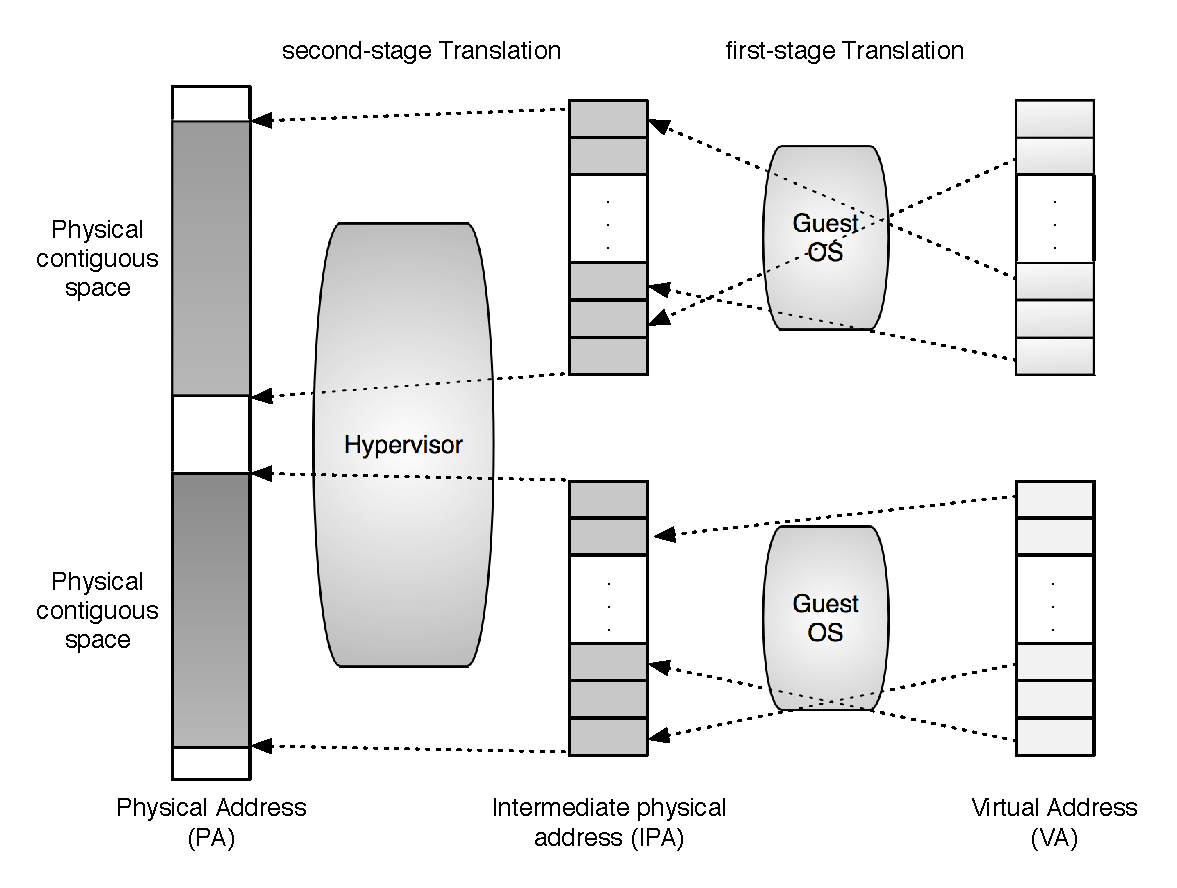
\includegraphics[width=0.6\textwidth]{chapter5/figures/tlb-hyper2}
	\caption{Virtual memory organization view of our hypervisor.}
	\label{fig:tlb-hyper}
\end{figure}


Typical hypervisors for cloud computing implement a complete paging mechanism. The hypervisor keeps a page table to map guest OSs to physical addresses. In these systems, the guest OS does not need to be entirely loaded into the main memory to be executed. In fact,  the hypervisor can implement an on-demand paging mechanism (swapping). Such a scheme reduces the memory usage since pages that have not been used recently can be stored in the swapping system. Additionally, it avoids the memory external fragmentation problem because the VMs do not need to be allocated contiguously in the physical memory. However, this approach has critical drawbacks for ESs. First of all, swapping systems and on-demand paging mechanisms impact real-time responsiveness. Additionally, some ESs do not support swapping due to storage restrictions. Moreover, a complete virtual memory management mechanism implies a more complex hypervisor and, consequently, a larger footprint and more processing requirements. 

A simplified virtual memory management mechanism brings some advantages to ESs. First, it avoids second-stage TLB misses keeping the VM entirely mapped at the TLB during its execution. Thus, RTOSs that do not implement virtual memory support will not suffer additional delays and jitter due to hypervisor paging management. Secondly, some ESs execute a limited number of virtual machines and some keep a static configuration during their execution. For these systems, memory fragmentation due to contiguous guest OS allocation is not a major problem. This implementation supports mapped devices directly, i.e., it can map non-continuous memory regions to a VM. Usually, such devices are mapped to specific physical addresses requiring a special mapping for guest access. For example, a VM may have mapped 32Mbytes of RAM to be loaded into the physical memory at 0x1000\_0000. If the same guest requires access to a memory mapped peripheral at physical address 0x1F00\_0800 the hypervisor must configure a second-stage TLB entry to match this address. Finally, a VM requires, at least, one TLB-entry to be mapped at the second-stage TLB, and an additional TLB-entry for each directly mapped peripheral. The M5150 has 32 TLB-entries. If the number of TLB-entries needed to map all VMs and peripheral on a system exceeds 32 entries, the hypervisor must reconfigure the TLB on each context-switching.  

\section{Interrupt Virtualization}
\label{section5:interrupt}

The MIPS VZ module allows to map an interrupt source directly to a guest OS avoiding hypervisor intervention. This mechanism is known as interrupt pass-through and it allows one to support directly mapped devices. Therefore, it does not share devices between guests, but allows a certain guest OS to have direct access. The main advantage of this technique is low overhead, which is close to non-virtualized systems in terms of throughput and latency. However, if an  interrupt occurs during the execution of any other guest OS, the hypervisor must decide between:

\begin{itemize}
    \item keep the interrupt masked and delay its delivery or;
    \item intercept the interrupt and reschedule the guest OSs.
\end{itemize}

This allows the implementation of different policies for interrupt control. For example, for low priority devices such as a serial port for a user console, the hypervisor may choose to keep the interrupt masked while in the supervisor mode. Thus, the guest OS will handle the interrupt only on its next execution (hypervisor scheduling quantum), resulting in a relatively long delay. This requires a large buffer queue in hardware or hardware flow control, otherwise, data may be lost. This arrangement is acceptable for low bandwidth, non interactive devices. Devices with higher priority or higher bandwidth may require hypervisor intervention to avoid long delays in the interrupt handling. To illustrate a typical scenario, suppose that a Linux guest has a directly mapped Ethernet device.  In this case, the hypervisor can keep the Ethernet interrupt unmasked to perform a context switch between guests when a network packet is received and the Linux guest is not executing.

\begin{figure}[!hbtp]
\centering
\subfigure[Interrupt delayed.]{
    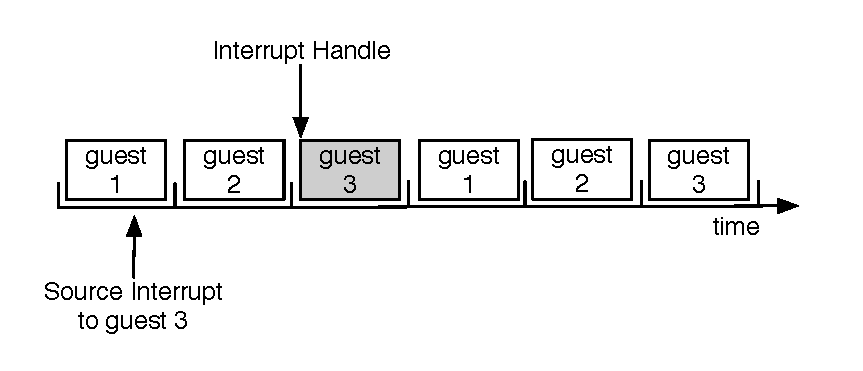
\includegraphics[width=.4\textwidth]{chapter5/figures/interruptdelay}
    \label{subfig:interruptdelayA}
}
\subfigure[Fast interrupt with recycled quantum.]{
    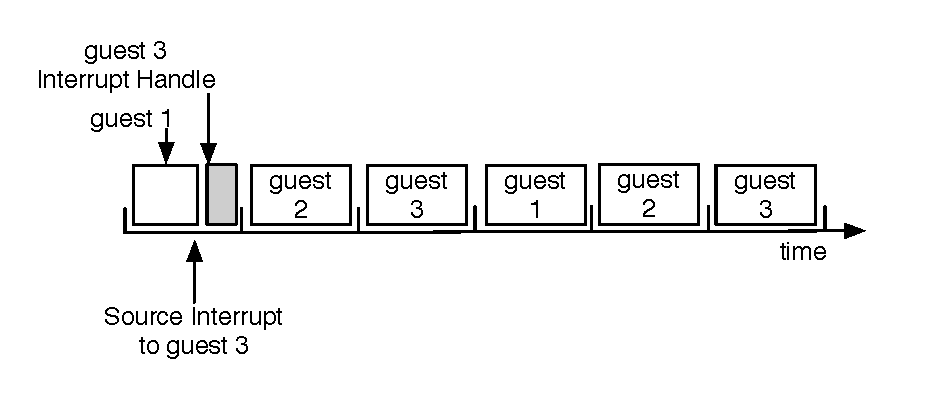
\includegraphics[width=.4\textwidth]{chapter5/figures/interrupt_short_quantum}
    \label{subfig:interruptdelayB}
}
\subfigure[Fast interrupt with reset quantum.]{
    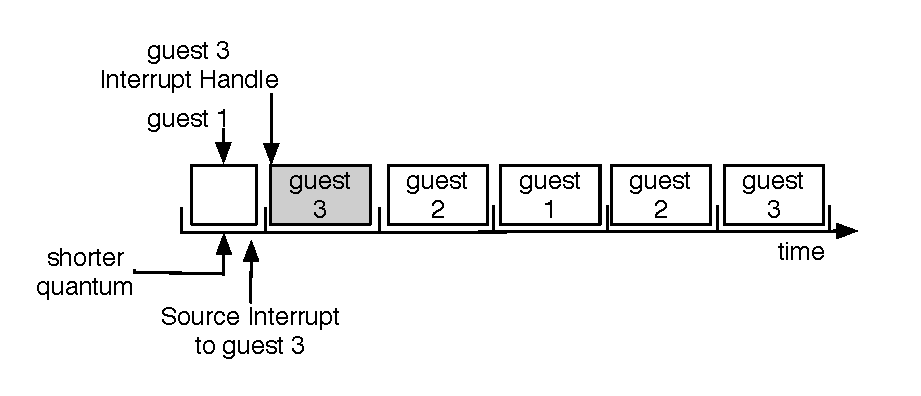
\includegraphics[width=.4\textwidth]{chapter5/figures/interrupt_new_quantum}
    \label{subfig:interruptdelayC}
}
\captionsetup{justification=centering}
\caption{Quantum scheduler scheme for interrupt delivery.}
\label{fig:interruptdelay}
\end{figure}


Figure \ref{fig:interruptdelay} depicts three guest OSs being scheduled in a round-robin policy with the three different quantum schemes for interrupt handling. Figure \ref{subfig:interruptdelayA} shows an interrupt targeted to the guest OS 3 being asserted during the execution of the guest OS 1. Without a proper hypervisor policy, the interrupt delivery will be delayed until the execution of the guest OS 3. In fact, the overhead is similar to a non-virtualized system since there is no hypervisor intervention. However, this causes a long delay to deliver the interrupt. This implementation was designed to use the interrupt pass-through mechanism, which allows for the coexistence of general-purpose OSs and RTOSs with minimal interrupt delivery delay. First, we studied two different schemes regarding the use of the scheduler quantum: recycle quantum and reset quantum. Figure \ref{subfig:interruptdelayB} shows a fast interrupt delivery approach, causing the preemption of the current guest OS and the dispatch of the guest which will execute during the time remaining in the same quantum. In Figure \ref{subfig:interruptdelayC}, the current quantum is shortened, and the dispatched guest will execute during an entire new quantum. Chapter \ref{section6:interruption-delay} presents the results and discussion about the implications of these different approaches. 

Independently of the quantum scheme adopted, our hypervisor accepts a set of rules to describe the behavior to address different interrupt sources. This set of rules is defined at design time. For each guest OS, the designers define which interrupts are directly mapped and, if an interrupt can induce the preemption of the current guest OS. Additionally, a higher priority guest OS can be marked to never be preempted by the hypervisor during its scheduler quantum. Table \ref{table:rules} shows a possible configuration for three guest OSs. Guest 1 has the timer and serial 1 interrupts directly mapped. The column Root Int describes which interrupts will trigger the hypervisor when the guest is not executing. In this case, the hypervisor will intercept serial 1, dispatching Guest 1. Guest 2 has the timer and serial 2 interrupt sources directly mapped. The hypervisor will intercept serial 2 interrupts when the guest is not executing only if the current guest is marked to be preempted. In the example, the hypervisor will preempt guest Linux 1 to deliver network interrupts to guest 2, but the same interrupts will be delayed if the guest 1 is executing. Thus, a high priority guest OS cannot be preempted by events from other guests, but only by the hypervisor scheduler. Our hypervisor provides a strong temporal isolation between guests, which is essential in ES virtualization if predictability of the RTOSs is a major concern. In addition, the flexibility of this approach allows the system to be configured for specific applications. Finally, our hypervisor always keeps the guest timer interrupt directly mapped, since it avoids hypervisor intervention during guest scheduling. 

\begin{table}[!hbtp]
\caption{Example of a set of interrupt rules for a system configured with three guest OSs.}
\label{table:rules}
\centering
\begin{tabular}{llll}
\hline
                                    &                                                       & \multicolumn{2}{c}{\textbf{Rules}}                                           \\ 
\multicolumn{1}{c}{\textbf{Guests}} & \multicolumn{1}{c}{\textbf{Direct Mapped Interrupts}} & \multicolumn{1}{c}{\textbf{Root Int}} & \multicolumn{1}{c}{\textbf{Preempt}} \\ \hline
Guest 1                               & Timer, Serial 1                                       & Serial 1                              & No                                   \\
Guest 2                              & Timer, Serial 2                                               & Serial 2                                  & Yes                                    \\
Guest 3                              & Timer, Network                               & Network                               & Yes                                    \\ \hline
\end{tabular}
\end{table}


\subsection{Virtual Interrupt}
\label{section5:virtual_interrupt}

The M5150 processor core supports an interrupt injection mechanism called virtual interrupt. Virtual interrupts are software generated and used when the hypervisor needs to inject interrupts in the guest OSs. Our hypervisor implements a secure inter-VM message passing mechanism described in Section \ref{chapter5:inter-vm} based on para-virtualization and virtual interrupt injection. 

%Descrever brevemente o mecanismo de injecao de interrupção.

\section{Inter-VM Communication}
\label{chapter5:inter-vm}

As explained in Subsection \ref{subsection4:comm}, the proposed virtualization model does not define a communication mechanism. However, it defines a hypercall interface for communication among VMs. Thus, this implementation adopts a message passing mechanism based on para-virtualization.  The hypervisor uses the VM identification number to route the messages among the VMs. The hypervisor requires the address, size and ID destination to route a message, which are discovered during the hypercall. Thus, the hypervisor does not make any assumptions about the message formatting; this is entirely the responsibility of the communicating guest OSs. For example, if a multi-task guest OS needs to demultiplex \cite{tanenbaum2011} incoming messages among different tasks, it may add a header to the message indicating the origin and destination task id. In this case, different guest OSs must agree about the header format.

\begin{figure}[!hbtp]
	\centering
	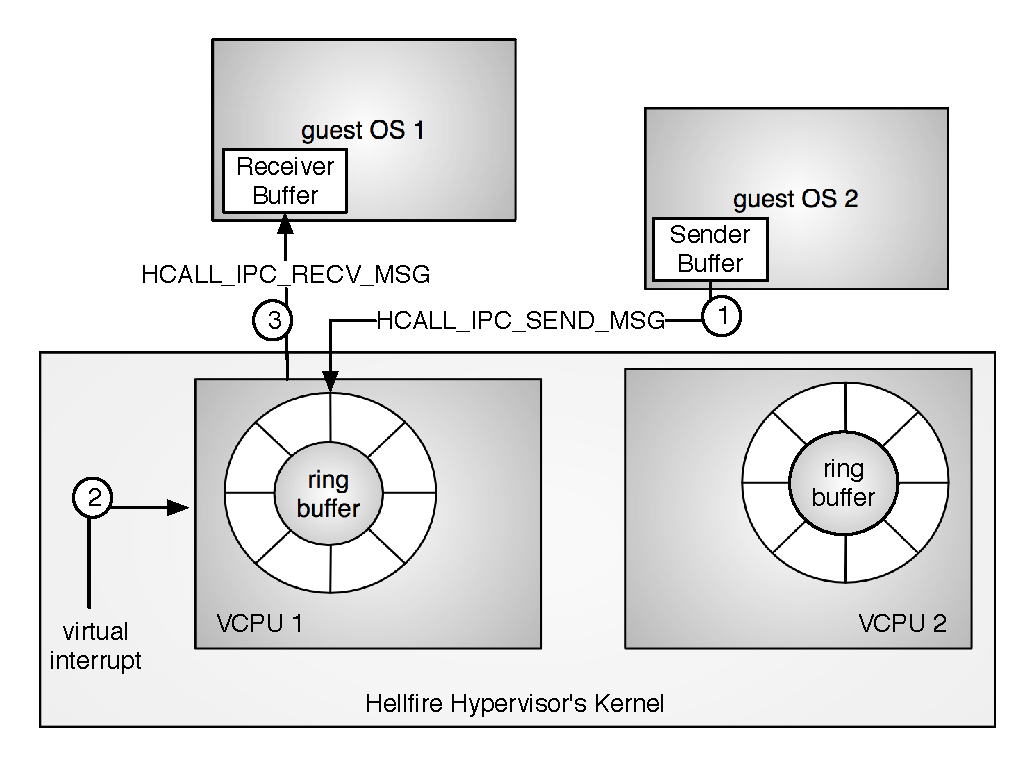
\includegraphics[width=0.5\textwidth]{chapter5/figures/intervm-comm}
	\caption{Example of inter-VM communication involving two guests.}
	\label{fig:intervm-comm}
\end{figure}

Each VCPU implements its incoming message queue as a circular buffer, statically allocated for performance purposes. A message targeting a determined VCPU will be copied to its queue, and the hypervisor will insert a virtual interrupt to the VCPU. The next time that the VCPU is executed it will handle the virtual interrupt and call the hypercall to retrieve the message. Figure \ref{fig:intervm-comm} describes the hypervisor behavior while redirecting messages between guests. The guest OS 2 invokes the HCALL\_IPC\_SEND\_MSG hypercall (1) causing a message copy from the guest's buffer to the ring buffer of the VCPU 1. After, the hypervisor injects a virtual interrupt (2) in the VCPU 1. In the next execution, the guest OS 1 will answer to the interrupt and executes the HCALL\_IPC\_RECV\_MSG hypercall. Thus, the hypervisor will copy the message from the ring buffer to the target buffer (3). 


\section{Engineering Effort to Support a Guest OS}

Due to the full-virtualization feature, to port a new guest OS to the Hellfire Hypervisor does not require any modification of the guest OS's kernel. However, it is important to highlight that the OS must be ported to the target platform. Thus, it must be able to execute natively on the hardware platform. To port an OS to a new processor or platform is a different job, and it is not necessarily related to virtualization. Thus, the designers must know some details about the memory mapping and platform resources required by the target OS. A guest OS requires specific memory regions, and it may depend on platform resources such as timer counters or other sources of interrupts. The hypervisor allows one to  describe the memory arrangement for each guest OS at design time. This description consists of mapping from IPA to PA (see Subsection \ref{subsection:hardware-assisted}) addresses that are written to the second-stage TLB by the hypervisor. The designers must choose the amount of main memory available to the guest OS based on the application and OS requirements. For example, 16MB of DRAM are enough to execute a minimal Linux distribution, while 64KB of DRAM are sufficient for a Hellfire OS guest with several tasks. Next, the designers must choose a contiguous area of physical memory to allocate to the guest OS. Additionally, the designers must determine which interrupts and peripherals will be directly mapped to the guest OS. Again, the arrangement between the source of interrupts and target guest OSs is described in a data structure at design time. In any case, the timer interrupt must at least be mapped to the guest OS, since this implementation does not provide timer emulation, i.e., each guest OS must receive its timer interrupts directly. Table \ref{table:rules} shows how the interrupt mapping can be described. 

\begin{table}[!hbtp]
\centering
\caption{Example of memory mapping for a Linux and a HellfireOS guests.}
\label{table:guestaddresses}
\begin{tabular}{
>{\columncolor[HTML]{FFFFFF}}l 
>{\columncolor[HTML]{FFFFFF}}l 
>{\columncolor[HTML]{FFFFFF}}l 
>{\columncolor[HTML]{FFFFFF}}l }
\hline \hline
                                                              & \multicolumn{3}{c}{\cellcolor[HTML]{FFFFFF}\textbf{Addresses}}                                                                                                               \\
                                                              & \multicolumn{1}{c}{\cellcolor[HTML]{FFFFFF}\textbf{VA}} & \multicolumn{1}{c}{\cellcolor[HTML]{FFFFFF}\textbf{IPA}} & \multicolumn{1}{c}{\cellcolor[HTML]{FFFFFF}\textbf{PA}} \\ \hline
\cellcolor[HTML]{FFFFFF}                                      & 0x8000\_0000                                            & 0x0000\_0000                                             & \textbf{0x1000\_0000}                                   \\
\multirow{-2}{*}{\cellcolor[HTML]{FFFFFF}\textbf{Linux}}      & 0xBF00\_0000                                            & 0x1F00\_0000                                             & 0x1F00\_0000                                            \\
\cellcolor[HTML]{FFFFFF}                                      & 0x8000\_0000                                            & 0x0000\_0000                                             & \textbf{0x1200\_0000}                                   \\
\multirow{-2}{*}{\cellcolor[HTML]{FFFFFF}\textbf{HellfireOS}} & 0xBF00\_0000                                            & 0x1F00\_0000                                             & 0x1F00\_0000                                            \\ \hline
\end{tabular}
\end{table}

Table \ref{table:guestaddresses} shows a valid memory mapping for a Linux and Hellfire OS guest. Both OSs are compiled to execute at the 0x8000\_0000 VA. Additionally, each OS require access to peripherals. Thus, a 4KB page is mapped at 0xBF00\_0000, where the peripherals mapping starts in the SEAD-3 development board (see Section \ref{section6:devboard}). Note that each guest requires, at least two TLB entries. The addresses 0x8000\_0000 and 0xA000\_0000 (including 0xBF00\_0000) correspond to the Kseg0 and Kseg1 memory segments, respectively, as shown in Figure \ref{fig:mips_memory}. These segments are fixed mapped and correspond to the 0x0000\_0000 physical address. However, when implementing the MIPS-VZ module, these addresses become IPA, and the hypervisor must map them to the PA. The PA column shows the 0x1000\_0000 and 0x1200\_0000 addresses highlighted since they correspond to the physical addresses where the guests are located in the memory. Additionally, for peripheral mapping the IPA and PA are the same because the hypervisor keeps the original addresses where the guest OSs expect to find the peripherals. 


\subsection{Linux and Hellfire OSs as Guests}

Most of the work to port an OS to the Hellfire Hypervisor is described in Tables \ref{table:rules} and \ref{table:guestaddresses}. However, some details must still be explained. Current Linux releases do not use periodic timer interrupts. In fact, when the OS is idle, it programs the timer interrupt to the next event, even if it will take several scheduler quanta, and executes the \textit{wait} instruction. This instruction will put the processor in the power saving mode. The processor comes up once an interrupt arrives. However, wait is a privileged instruction that must be emulated by the hypervisor. Emulating this instruction means to check when the next OS timer interrupt is programmed to happen and to program an event in the hypervisor to insert a virtual interrupt in the guest. However, the current implementation does not support emulation of this instruction. Thus, the Linux kernel was configured to use the periodic timer interrupt technique. Note that this is not an OS modification, since it was not needed to write kernel patches. Instead, both ways to use the timer interrupts are kernel features and they can be selected during kernel initialization. Finally, modifications were made to the Linux kernel to improve its performance once executed as a guest. This is better explained in Section \ref{section6:linuxport}.

Hellfire OS has fewer restrictions than Linux when virtualized since it is a simpler operating system. However, an initial port to the M5150 processor had to be done before it was virtualized. Once virtualized, para-virtualized communication drivers were then implemented to allow inter-VM communication. 

%The only board peripheral supported is the serial port used for communication.

\section{Current Hypervisor Restrictions}

Similar to any other implementation based on a theoretical model, the proposed hypervisor faces some limitations. The first limitation is that the M5150 is a single-core processor. The model proposes to support homogeneous multicore processors. The decision for this processor core was based on availability. The M5150 was one of the first MIPS processors, released in early 2013, implementing the MIPS-VZ technology. Additionally, it was the first MIPS core supporting MIPS-VZ module available to the GSE group. As a single-core processor, mutex or spinlocks are not required in the hypervisor since there are no concurrent executions on its kernel. A consequence is a simpler hypervisor kernel. Finally, it is important to highlight that this is a limitation imposed by the hardware platform that can be overcome when multicore processors become available.

Despite the overhead imposed by share devices, they are important in different situations. Because many guest OSs may require communication with the external world, the only solution is to implement a switching layer at the hypervisor level and para-virtualized device drivers to the VMs. The current stage of this implementation does not support any shared device, e.g. Ethernet. However, the implementation of a shared device is a matter of engineering effort since the para-virtualized interface between guest OSs and the hypervisor is already supported for inter-VM communication. The optimization and techniques to support shared devices is a future work.

The inter-VM communication implemented as a message passing mechanism is a secure and effective communication channel. However, as shown in Section \ref{subsection:intervm}, it imposes an excessive overhead to the system. Significant improvements can be achieved using a shared memory communication mechanism that is not available at this moment. 

The RT-VM concept provides strong temporal isolation among VMs. Additionally, it avoids the hierarchical scheduling problem. A restriction of the RT-VM is that it does not provide a compatible software environment for legacy software libraries. This means, any implementation must be build from scratch, impacting time-to-market and costs. However, this is a model restriction since it does not provide any tool or resource to avoid the problem. A practical implementation may avoid this problem porting a RTOS to execute as a guest in the RT-VM with its scheduler disabled, consequently, executing just one task. Thus, the application can use the RTOS's legacy libraries, but without concurrent tasks. 

The Hellfire Hypervisor was built from scratch avoiding any proprietary or open-source external library which makes it the propriety of the GSE group. However, this results in an important drawback: all engineering efforts must be from the university group. Different from several other open-source hypervisors those count on contributions from different groups, the Hellfire Hypervisor is entirely the responsibility of the GSE group. As a result, the current implementation only supports  Linux/MIPS and Hellfire RTOS guests. Additionally, there are limitations caused by the lack of engineering efforts because of  the small number of engineers working on the project. However, the Hellfire Hypervisor is planned to be released as an open-source software in early 2016. 

%1 linux guest

\section{Final Considerations}

An important question about theoretical models is how practical is it for them to be implemented on a hardware/software platform. This implementation demonstrated that the model can be implemented with relatively simple algorithms and data structures help to keep a small footprint. A factor that contributed to the simplification of the hypervisor was the M5150's hardware-assisted virtualization, especially the support for memory and MIPS CP0 virtualization. The footprint and performance results are analyzed in Chapter \ref{chapter6:evaluation}. The only feature not implemented was the multi-core support because the target processor is single-core. The absence of multi-core support simplified the hypervisor's kernel because it avoided the need for mutex or spinlocks. Other restrictions, like the lack of shared devices, concerns to the limited time and number of engineers working on the project, which can be overcome with more engineering effort. It is fair to conclude that the presented implementation is a suitable representation of the virtualization model proposed in the Chapter \ref{chapter:vtmodel}.



































